\chapter{Experiments and Results} \label{chap3}

In this section, we describe the experimental results of our model along with the parameters required to reproduce those results. We also describe baselines that we compare our model with, along with their parameters.

\section{Dataset Description}

We use the real-world traffic volumes of Dublin city streets collected using the SCATS (Sydney Coordinated Adaptive Traffic System)\cite{scats} system over a three-month period. The SCATS system is used in Dublin as an adaptive urban traffic management system that synchronizes traffic signals and optimizes traffic flow across the entire city.

The dataset consists of traffic volumes from the 825 sensors at all key intersections in Dublin city, sampled at a frequency of 1 hour during a time period of 3 months, from October 1, 2023, to December 31, 2023. The dataset contains the latitudinal and longitudinal geographical coordinates along with the timestamped total volume of traffic detected by each detector in the one-hour period.

We also verify the model for the task (iii) on SUMO\cite{sumo} TAPASCologne scenario\cite{tapas}, which is a simulation configuration that describes the traffic dynamics of Cologne city in Germany for a day. The scenario is publicly available on the official SUMO website and was created using mobility demand data based on information about the traveling habits of citizens and information about the infrastructure of the area they live in. Since this testing is manual, we run a limited number of tests, where we change an edge and process the simulation based on the default minimal travel time routing before and after the change and observe the deviation between the simulation and our results.

\begin{figure}[htbp]
  \centering
  \includegraphics[width=0.75\textwidth]{dataset.png}
  \caption{Snapshot of sensor locations plotted along with road network from Overpass API}
  \label{fig:dataset}
\end{figure}


\section{Model Parameters}

For all experiments, we set hyperparameters $T = 3$, which is the number of consecutive timesteps to consider for prediction and imputation tasks. For all tasks, we optimize the model input by assuming the locality of traffic within such a timespan and that any changes to a particular node are only dependent on nodes "close" to it. Formally, during training, we train on sub-graphs consisting of the node clusters instead of the entire graph all at once. Specifically, a subgraph is generated by choosing a node $u$ at random and then selecting all nodes that are at a distance less than $\sigma$ to it, specifically for $G(V, E)$, $G_{\text{sub}} = G\{v \in V \; | \; \text{dist}(u, v) < \sigma\}$. For our experiments, we set $\sigma$ as $2.5\ km$, which is a reasonable expectation as clusters usually contain 20 to 30 nodes within this range.

After sampling, as stated before, we use an 80-20 test-train split, i.e., the model is trained on 80\% of the samples, and then performance is verified on new unseen data that comprises 20\% of the samples. The data is then modified based on the task at hand. For imputation, we followed MCAR (Missing Completely at Random) distribution and randomly masked values both spatially and temporally, following a parameter defined as the miss rate, we tested our model on miss rates of 10\%, 20\%, 30\%, and 40\%. For prediction, we use the full data of three timesteps to predict the fourth step by basically masking the values along the last timestep dimension. For the re-assignment task, i.e., task (iii), we only consider one timestep and re-assign values for that same timestep but with modified spatial geometry.

\section{Baselines}

We compare our \modelname\ model with a number of different existing approaches across different domains, including different mathematical analysis and deep learning techniques used popularly for these tasks.

One of the simplest approaches for imputation is \textit{KNN}. Similarly, for prediction, \textit{ARIMA}\cite{arima} stands for AutoRegressive Integrated Moving Average is used. Matrix factorization methods like \textit{TRMF}\cite{trmf} (Temporal Regularized Matrix Factorization) use latent factors for predictions, and its modification \textit{BTRMF}\cite{btrmf} (Bayesian Temporal Regularized Matrix Factorization) extends TRMF with a Bayesian framework. For both these methods, we use rank $= 10$, $1000$ burn-in iterations, and $200$ Gibbs iterations.

\textit{LRTC-TNN}\cite{lrtc} (Low-Rank Tensor Completion with Truncated Nuclear Norm) is a method for tensor completion. It uses parameters $\rho = 1e-5$, $\theta = 0.25$, and $\epsilon = 1e-4$. \textit{BGCP} (Bayesian Gaussian Process Factorization) is another method that utilizes Bayesian inference. For BGCP, we use similar burn-in and Gibbs iterations and set rank $= 30$. It is worth noting that these model baselines are only applicable to task (i) and task (ii) and not to task (iii) since they were not built with that task as a consideration.

Finally, we use deep learning methods. For imputation, we employed the \textit{Denoising AutoEncoder} (DAE)\cite{dae} model, which is effective in learning meaningful representations of the data while handling missing values. For prediction tasks, we utilized an \textit{LSTM}\cite{lstm} (Long Short-Term Memory) model as LSTM networks are well-suited for capturing temporal dependencies in sequential data.

\section{Evaluation metrics}

In order to evaluate the performance of the different methods and compare them, we use RMSE (Root Mean Squared Error) and MAPE (Mean Absolute Percentage Error). These metrics are defined as:


\[
\text{RMSE} = \sqrt{\frac{1}{n} \sum_{i=1}^{n} (y_i - \hat{y}_i)^2}
\]

\[
\text{MAPE} = \frac{1}{n} \sum_{i=1}^{n} \left| \frac{y_i - \hat{y}_i}{y_i} \right| \times 100\%
\]

where \( y_i \) represents the true value, \( \hat{y}_i \) represents the predicted value, and \( n \) is the number of samples.

\section{Results}

We evaluated the performance of our model on different tasks and compared them with other popular models used in the domain.

\subsection{Prediction}
For the prediction task, we tested the models for predicting traffic volumes at the next timestep, i.e., the forecasting $\delta = 1$, at the third time step, i.e., $\delta = 3$ and the fifth timestep in the future, i.e., $\delta = 5$. This scenario of predicting the next time step requires a mask consisting of all the $T_{n+1}$ values missing, i.e., 0. We prepare a mask similarly for other time horizons. Thus, prediction here is treated as a strict MNAR (Missing Not At Random) subcategory of imputation.

The MAPE and RMSE plots of prediction tasks on different horizons are shown in Fig. \ref{fig:mape_pred} and Fig. \ref{fig:rmse_pred}, respectively. We observe that in general, as the $\delta$, i.e., the time horizon to predict in the future, increases, both metrics worsen with MAPE falling 5-10\% from $\delta=1$ to $\delta=3$, i.e., we see a stronger short term accuracy but face some challenges with long-term prediction, across all models. This trend is common in time-series forecasting, where predictive accuracy decreases as the prediction horizon extends. The primary reasons for this decline include the increasing uncertainty and the influence of unpredictable external factors, such as accidents or weather changes. We see that ARIMA performs worst, which is to be expected since it is the simplest of mathematical models among the baselines we consider. The other matrix factorization and Bayesian models like TRMF, BTRMF, and BTMF perform better, but given that they are strictly mathematical models, they (i) fail to capture the intricate traffic dynamics that a deep learning model can and (ii) use only the time-series traffic data and not the graph topology and external factors that our model considers like weather, etc. Finally, we see that LSTMs are close with slightly (2-3\%) worse performance, which could be attributed to a lack of knowledge of graph topology that we incorporate in our model through $Node2Vec$.

\begin{figure}[H]
    \centering
    \begin{subfigure}{1\textwidth}
        \centering
        \includegraphics[width=1\linewidth]{mape_pred.eps}
        \caption{MAPE on prediction task for different deltas (timesteps to predict ahead)}
        \label{fig:mape_pred}
    \end{subfigure}
    
    \begin{subfigure}{1\textwidth}
        \centering
        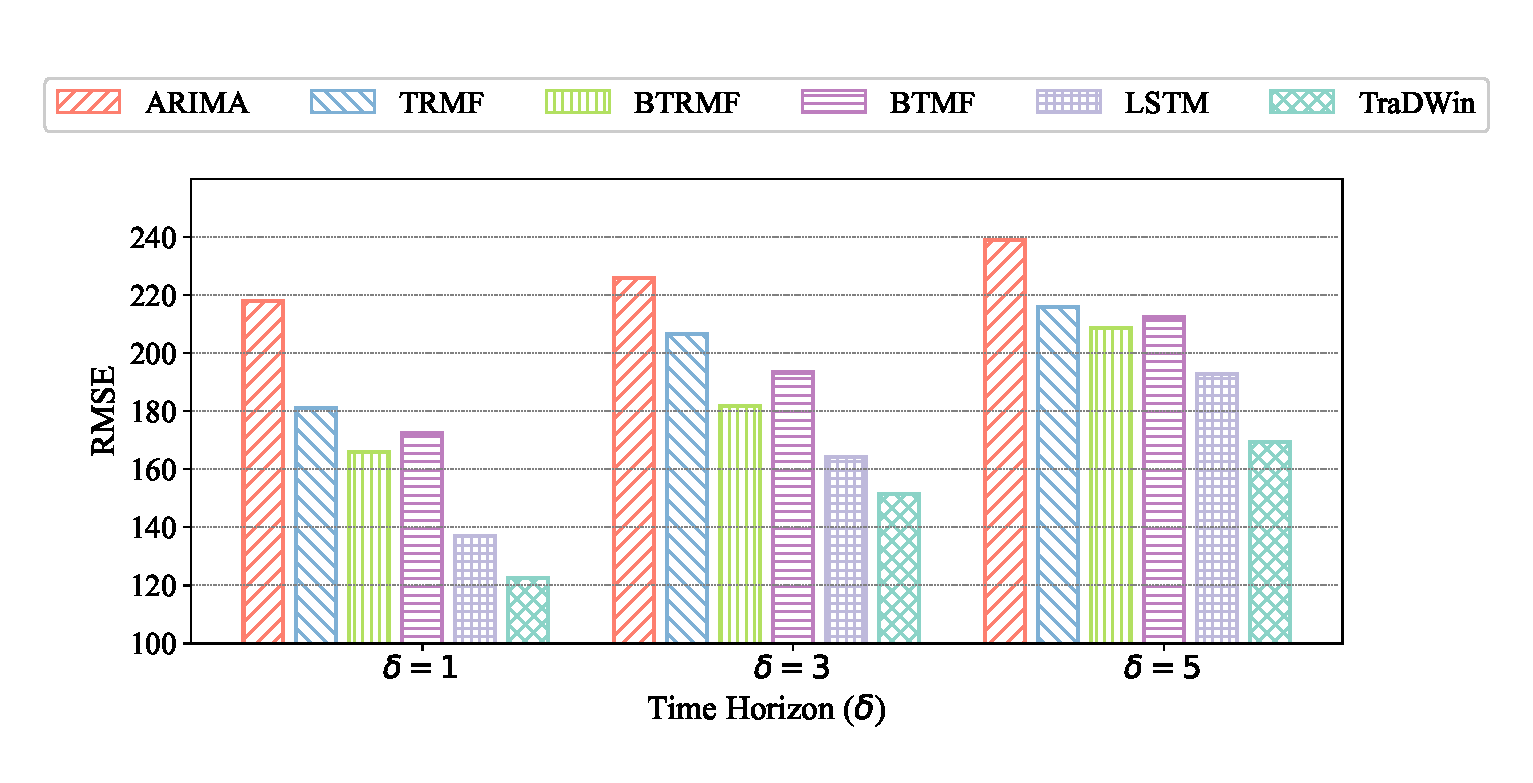
\includegraphics[width=1\linewidth]{rmse_pred.eps}
        \caption{RMSE on prediction task for different deltas (timesteps to predict ahead)}
        \label{fig:rmse_pred}
    \end{subfigure}
    \caption{MAPE and RMSE on prediction task for different deltas}
    \label{fig:pred_comparison}
\end{figure}

\subsection{Imputation}

Next, we evaluate performance on the imputation task. For this task, we have considered the MCAR (Missing Completely At Random) distribution and compared the models at five missing rates of $10\%$, $20\%$, $30\%$, $40\%$, and $50\%$. The performance of different models measured using MAPE and RMSE is shown in Fig. \ref{fig:imput}. We see that the conventional methods, like KNN, perform poorly to more specialized approaches, which is to be expected since KNN is not enough to capture the intricate traffic dynamics. The matrix factorization and Bayesian methods, which are TRMF, BTRMF, and BGCP, work slightly better, with deep learning methods like DAE following ahead, though since they deal with only traffic data time series with no information on topology, they have an 8-13\% worse off performance than our model. Tensor completion based model like LRTC-TNN is close to our \modelname\ in for low missing rates, but we see that it does not scale as well with increasing missing rates, possibly because too much data is lost for reliable tensor completion, which a deep learning model can still handle, due to being able to learn more complex relationships in data and having knowledge of graph topology and other external factors. Moreover, it is worth noting that LRTC-TNN is an MCAR imputer and not applicable to task (iii), so it is not generalized enough for our use case. For all models, we see that the accuracy of imputations decreases with higher missing rates due to the reduced amount of contextual information available. This is a common challenge in data imputation, where fewer data points make it harder to discern underlying patterns accurately. 

We also observe that \modelname\ performs worse on task (i) than task (ii) by around 4\%. One primary reason for this, as we suspect, could be that GAIN, which was originally designed for MCAR (Missing Completely At Random) imputation, does not generalize well to MNAR imputation scenarios. Another possible reason could be the subgraph-based computation method that we use, where nodes at the corners of the subgraph do not have adequate spatial and temporal information about their neighbors. Still, we observe that our model performs reasonably and delivers comparable results for being a generalized model.

\begin{figure}[H]
  \centering
  \begin{subfigure}{1\textwidth}
    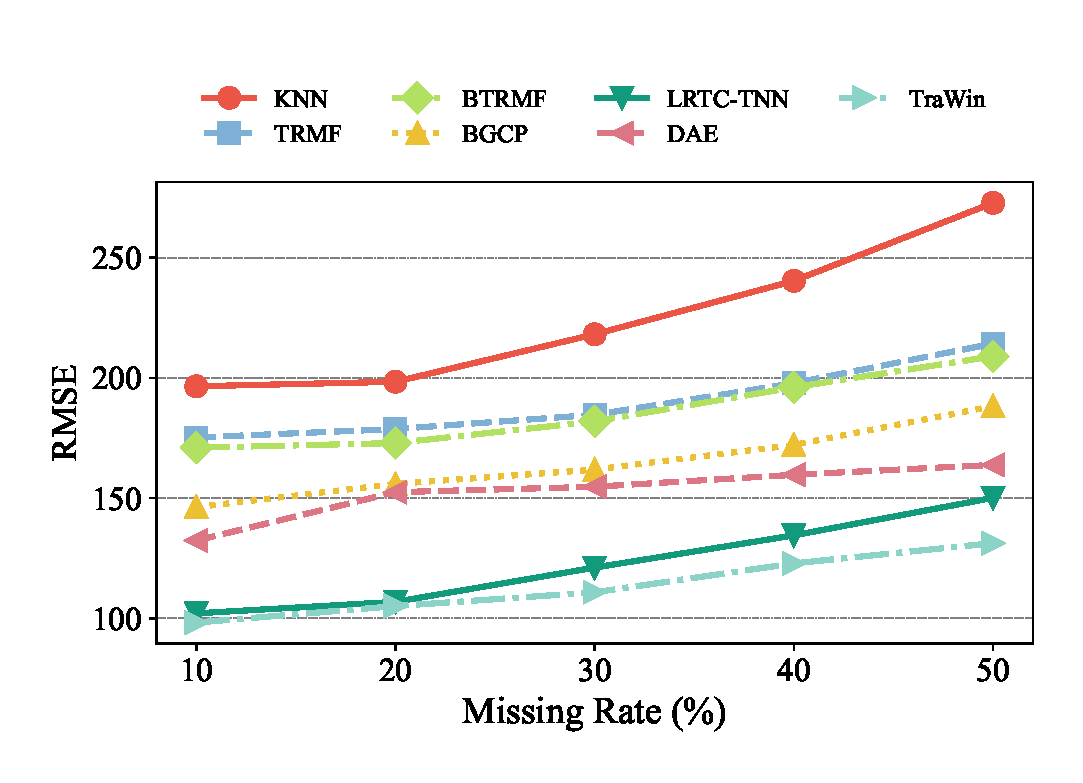
\includegraphics[width=\linewidth]{rmse_imput.eps}
    \caption{RMSE of different models on imputation task}
    \label{fig:mape_imput}
  \end{subfigure}
  
  \begin{subfigure}{1\textwidth}
    \includegraphics[width=\linewidth]{mape_imput.eps}
    \caption{MAPE of different models on imputation task}
    \label{fig:rmse_imput}
  \end{subfigure}
  \caption{Imputation comparison for different missing rates}
  \label{fig:imput}
\end{figure}

\subsection{Re-assignment}

Finally, on the re-assignment task, which is a new task that we address in our paper and is not conventionally seen in contemporary literature, we essentially train the model for MNAR (Missing Not At Random) imputation scenarios with the central node cluster missing. This effectively makes the model learn how to assign traffic to node clusters given neighbor node information. Based on this training task, we achieved a MAPE of $13.47\%$ and RMSE of $109.90$. Note that the other baselines considered for prediction and imputation are not applicable to this without changes to their model architecture, so there is no comparison with contemporary models. Moreover, the de-facto way to solve this problem, as we have seen in our literature review, has been simulations like SUMO\cite{sumo} and Vissim\cite{vissim}. We, too, use those to compare and test our model on the TAPASCologne scenario using SUMO, which is a traffic simulation engine with the configuration described previously. The results of our model on this task are shown in Table. \ref{reassign_table}. We observe that the model achieves a MAPE of $13.47\%$ on the Dublin SCATS dataset and $15.06\%$ on the TAPASCologne scenario, which demonstrates that the model can, with reasonable accuracy, learn to solve the traffic assignment problem on node clusters. Further, we tried to evaluate how our model's performance scales with the number of modifications, i.e., how much we can alter the original graph so that the model is still viable to use for re-assignment. In Fig. \ref{fig:edge_modif}, we show a comparison of MAPE and RMSE with the number of edges modified. We see that performance declines steadily from $13.47\%$ at $1$ change to $31.91\%$ at five changes. So, altering more of the graph leads to a decline in performance, with the drop being significant and sharp after $3$ modifications. A possible reason for this could be the mass masking strategy we use to train the model for the task (iii). For five modifications, too many of the neighboring nodes are masked, leading to a large loss of contextual information that knowledge of graph representation does not compensate enough.

\begin{figure}[H]
    \centering
    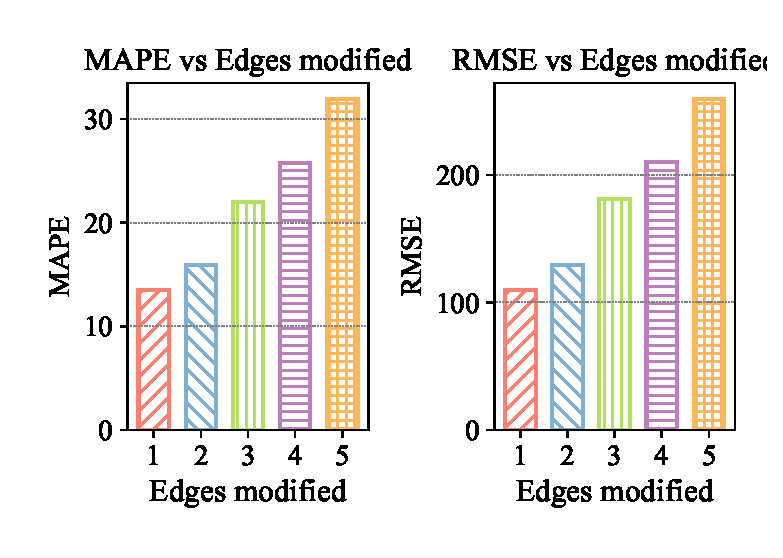
\includegraphics[width=0.8\linewidth]{modif.eps}
    \caption{MAPE and RMSE on re-assignment task vs number of edges modified}
    \label{fig:edge_modif}
\end{figure}

\begin{table}[]
\centering
\caption{Performance on re-assignment task (1 edge change) for different datasets}
\label{reassign_table}
\begin{tabular}{lcc}
\toprule
Dataset & MAPE (\%) & RMSE \\
\midrule
Dublin SCATS\cite{dublin_scats} & 13.47 & 109.90 \\
TAPASCologne\cite{tapas} & 15.06 & 23.34 \\
\bottomrule
\end{tabular}
\end{table}